\documentclass[a4paper,14pt]{extarticle}

% Путь до папки с общими шаблонами
\newcommand{\pathToCommonFolder}{/home/denilai/Desktop/LaTeX/Common}
% Название работы в титуле
\newcommand{\workname}{Отчет по практической работе №5}
% Название дисциплины в титуле
\newcommand{\discipline}{Теория автоматов}
% Название кафедры в титуле
\newcommand{\kafedra}{Кафедра Вычислительной техники}
% Тема работы в титуле
\newcommand{\theme}{Сложение чисел с плавающей точкой}
% Должность преподавателя в титуле
\newcommand{\rang}{ассистент}
% ФИО преподавателя в титуле
\newcommand{\teacherfio}{А.~С.~Боронников}


\usepackage{tabularx}

\usepackage{booktabs}
\newcolumntype{b}{X}
\newcolumntype{s}{>{\hsize=.5\hsize}X}
\newcommand{\heading}[1]{\multicolumn{1}{c}{#1}}

% Вставка заготовки преамбулы
% Этот шаблон документа разработан в 2014 году
% Данилом Фёдоровых (danil@fedorovykh.ru) 
% для использования в курсе 
% <<Документы и презентации в \LaTeX>>, записанном НИУ ВШЭ
% для Coursera.org: http://coursera.org/course/latex .
% Исходная версия шаблона --- 
% https://www.writelatex.com/coursera/latex/5.3

% В этом документе преамбула

% Для корректного использования русских символов в формулах
% пакеты hyperref и настройки, связанные с ним, стоит загуржать
% перед загрузкой пакета mathtext



% поддержка русских букв
% кодировка шрифта
%\usepackage[T2A]{fontenc} 
\usepackage{pscyr}

% использование ненумеровонного абзаца с добавлением его в содержаниеl

\newcommand{\anonsection}[1]{\section*{#1}\addcontentsline{toc}{section}{#1}}
\newcommand{\sectionunderl}[1]{\section*{\underline{#1}}}


% настройка окружения enumerate
\usepackage{enumitem}
\setlist{noitemsep}
\setlist[enumerate]{labelsep=*, leftmargin=1.5pc}

\usepackage{hyperref}

% сначала ставить \usepackage{extsizes} % Возможность сделать 14-й шрифт
% для корректной установки полей вставлять преамбулу следует в последнюю очередь (но перед дерективой замены \rmdefault)
\usepackage[top=20mm,bottom=25mm,left=35mm,right=20mm]{geometry} % Простой способ задавать поля

\hypersetup{				% Гиперссылки
	unicode=true,           % русские буквы в раздела PDF
	pdftitle={Заголовок},   % Заголовок
	pdfauthor={Автор},      % Автор
	pdfsubject={Тема},      % Тема
	pdfcreator={Создатель}, % Создатель
	pdfproducer={Производитель}, % Производитель
	pdfkeywords={keyword1} {key2} {key3}, % Ключевые слова
	colorlinks=true,       	% false: ссылки в рамках; true: цветные ссылки
	linkcolor=red,          % внутренние ссылки
	citecolor=black,        % на библиографию
	filecolor=magenta,      % на файлы
	urlcolor=blue           % на URL
}

%%% Работа с русским языком
\usepackage{cmap}					% поиск в PDF
\usepackage{mathtext} 				% русские буквы в формулах
\usepackage[T2A]{fontenc}			% кодировка
\usepackage[utf8]{inputenc}			% кодировка исходного текста
\usepackage[english,russian]{babel}	% локализация и переносы
\usepackage{indentfirst}
\frenchspacing

%для изменения названия списка иллюстраций
\usepackage{tocloft}


\renewcommand{\epsilon}{\ensuremath{\varepsilon}}
\renewcommand{\phi}{\ensuremath{\varphi}}
\renewcommand{\kappa}{\ensuremath{\varkappa}}
\renewcommand{\le}{\ensuremath{\leqslant}}
\renewcommand{\leq}{\ensuremath{\leqslant}}
\renewcommand{\ge}{\ensuremath{\geqslant}}
\renewcommand{\geq}{\ensuremath{\geqslant}}
\renewcommand{\emptyset}{\varnothing}

% Изменения параметров списка иллюстраций
\renewcommand{\cftfigfont}{Рисунок } % добавляем везде "Рисунок" перед номером
\addto\captionsrussian{\renewcommand\listfigurename{Список иллюстративного материала}}

\newcommand{\tm}{\texttrademark\ }
\newcommand{\reg}{\textregistered\ }


%%% Дополнительная работа с математикой
\usepackage{amsmath,amsfonts,amssymb,amsthm,mathtools} % AMS
\usepackage{icomma} % "Умная" запятая: $0,2$ --- число, $0, 2$ --- перечисление

%% Номера формул
%\mathtoolsset{showonlyrefs=true} % Показывать номера только у тех формул, на которые есть \eqref{} в тексте.
%\usepackage{leqno} % Нумереация формул слева

%% Свои команды
\DeclareMathOperator{\sgn}{\mathop{sgn}}

%% Перенос знаков в формулах (по Львовскому)
\newcommand*{\hm}[1]{#1\nobreak\discretionary{}
{\hbox{$\mathsurround=0pt #1$}}{}}


% отступ для первого абзаца главы или параграфа
%\usepackage{indentfirst}

%%% Работа с картинками
\usepackage{graphicx}  % Для вставки рисунков
\graphicspath{{images/}{screnshots/}}  % папки с картинками
\DeclareGraphicsExtensions{.pdf,.png,.jpg}
\setlength\fboxsep{3pt} % Отступ рамки \fbox{} от рисунка
\setlength\fboxrule{1pt} % Толщина линий рамки \fbox{}
\usepackage{wrapfig} % Обтекание рисунков текстом

%%% Работа с таблицами
\usepackage{array,tabularx,tabulary,booktabs} % Дополнительная работа с таблицами
\usepackage{longtable}  % Длинные таблицы
\usepackage{multirow} % Слияние строк в таблице

%%% Теоремы
\theoremstyle{plain} % Это стиль по умолчанию, его можно не переопределять.
\newtheorem{theorem}{Теорема}[section]
\newtheorem{proposition}[theorem]{Утверждение}

\theoremstyle{plain} % Это стиль по умолчанию, его можно не переопределять.
\newtheorem{work}{Практическая работа}[part]


 
 
\theoremstyle{definition} % "Определение"
\newtheorem{corollary}{Следствие}[theorem]
\newtheorem{problem}{Задача}[section]
 
\theoremstyle{remark} % "Примечание"
\newtheorem*{nonum}{Решение}



%%% Программирование
\usepackage{etoolbox} % логические операторы

%%% Страница

%	\usepackage{fancyhdr} % Колонтитулы
% 	\pagestyle{fancy}
%   \renewcommand{\headrulewidth}{0pt}  % Толщина линейки, отчеркивающей верхний колонтитул
% 	\lfoot{Нижний левый}
% 	\rfoot{Нижний правый}
% 	\rhead{Верхний правый}
% 	\chead{Верхний в центре}
% 	\lhead{Верхний левый}
%	\cfoot{Нижний в центре} % По умолчанию здесь номер страницы

\usepackage{setspace} % Интерлиньяж
\onehalfspacing % Интерлиньяж 1.5
%\doublespacing % Интерлиньяж 2
%\singlespacing % Интерлиньяж 1

\usepackage{lastpage} % Узнать, сколько всего страниц в документе.

\usepackage{soul} % Модификаторы начертания


\usepackage[usenames,dvipsnames,svgnames,table,rgb]{xcolor}


\usepackage{csquotes} % Еще инструменты для ссылок

%\usepackage[style=authoryear,maxcitenames=2,backend=biber,sorting=nty]{biblatex}

\usepackage{multicol} % Несколько колонок

\usepackage{tikz} % Работа с графикой
\usepackage{pgfplots}
\usepackage{pgfplotstable}

% модуль для вставки рыбы
\usepackage{blindtext}

\usepackage{listings}
\usepackage{color}


% для поворота отдельной страницы. Использовать окружение \landscape
\usepackage{pdflscape} 
\usepackage{rotating} 


\definecolor{mygreen}{rgb}{0,0.6,0}
\definecolor{mygray}{rgb}{0.5,0.5,0.5}
\definecolor{mymauve}{rgb}{0.58,0,0.82}


% пример импорта файла
%\lstinputlisting{/home/denilai/repomy/conf/distributions}

\lstset{
	language=Python,
	basicstyle=\footnotesize,        % the size of the fonts that are used for the code
	numbers=left,                    % where to put the line-numbers; possible values are (none, left, right)
	numbersep=5pt,                   % how far the line-numbers are from the code
	numberstyle=\tiny\color{mygray}, % the style that is used for the line-numbers
	stepnumber=2,                    % the step between two line-numbers. If it's 1, each line will be numbered
	% Tab - 2 пробела
	tabsize=2,    
	% Автоматический перенос строк
	breaklines=true,
	frame=single,
	breakatwhitespace=true,
	title=\lstname 
}



% установка размера шрифта для всего документа
%\fontsize{20pt}{18pt}\selectfont
\usepackage{extsizes} % Возможность сделать 14-й шрифт

\author{Кирилл Денисов}
\title{Практическая работа №5}
\date{\today}

% установка полуторного интервала
% \usepackage{setspace}  
% \onehalfspacing

% использовать Times New Roman
\renewcommand{\rmdefault}{ftm}


\begin{document}
	\thispagestyle{empty}
	
	% Вставка первого титульного листа
	%\newcounter{withouttheme}

%\setcounter{withouttheme}{<n>} установить значение счетчика  withouttheme для определения, нужна ли тема
%    {0} - нужна
%    {1} - не нужна

%\setcounter{withoutsubmissiondate}{<n>} установить значение счетчика  withoutsubmissiondate для определения, нужна ли дата представления к защите
%     {0} - нужна
%     {1} - не нужена
\begin{center}
	\begin{figure}[h!]
		\begin{center}
		%\vspace{-10ex}
		
\includegraphics[width=0.17\linewidth]{\pathToCommonFolder/gerb}
		%\caption{}\label{pic:first}
		%	\vspace{5ex}
		\end{center}	
	\end{figure}
 	\small	МИНОБРНАУКИ РОССИИ \\
	Федеральное государственное бюджетное образовательное учреждение\\
						высшего образования\\
\normalsize					
\textbf{«МИРЭА – Российский технологический университет»\\
						РТУ МИРЭА}\\
						\noindent\rule{1\linewidth}{1pt}\\
       Институт информационных технологий\\ %\vspace{2ex}
					\kafedra\\
		\vspace{3ex}
			\large \textbf{\workname}  \\
		%\vspace{1ex}
						по дисциплине\\ «\discipline» \\
		\vspace{3ex}
		\ifnum \value{withouttheme}=0 {
			\textbf{Тема работы:}\\ <<\theme>>
		}
		\else {}
		\fi
\vspace{10ex}
\small
\begin{table}[h!]
\begin{tabular}{lp{0.6\linewidth}l}
	\textbf{Выполнил:} & студент группы ИВБО-02-19 & \\ 
	& & \studentfio \\%Д.~Н.~Федосеев\\%А.~М.~Сосунов\\%К.~Ю.~Денисов\\%И.~А.~Кремнев
	\textbf{Принял:} & \rang & \\
	& & \teacherfio \hfill\\
\end{tabular}
\end{table}
\end{center}
\ifnum \value{withoutsubmissiondate}=0 {
	\begin{flushleft}
		Работа представлена к защите <<\rule{3ex}{1pt}>>\rule{10ex}{1pt} 202\rule{1ex}{1pt} г.\hfill
	\end{flushleft}
\else {}
\fi

\normalsize
\begin{center}	
\vfill
Москва 2022
\end{center}

	
	\newpage
	\tableofcontents
	\newpage
	
\section{Общее строение автомата}
В любом устройстве обработки цифровой информации можно выделить два основных блока – операционный автомат (ОА) и управляющий автомат (УА). Операционный автомат (ОА) служит для хранения слов информации, выполнения набора микроопераций и вычисления значений логических условий, т.е. операционный автомат является структурой, организованной для выполнения действий над информацией. Микрооперации, выполняемые ОА, задаются множеством \textit{управляющих} сигналов $Y\left\{y_1,....,y_M\right\}$, с каждым из которых отождествляется определенная микрооперация.

Значения логических условий, вычисляемые в операционном автомате, отображаются множеством \textit{осведомительных} сигналов $X=\left\{x_1,...,x_L\right\}$, каждый из которых отождествляется с определенным логическим условием.

Управляющий автомат (УА) генерирует последовательность управляющих сигналов, предписанную микропрограммой и соответствующую значениям логическим условий. Управляющий автомат задает порядок выполнения действий в ОА, вытекающий из алгоритма выполнения операций. Наименование операции, которую необходимо выполнить в устройстве, определяется кодом g операции, поступающим в УА извне. 

В отличие от УА с жесткой логикой, закон функционирования которого обеспечивается определенным образом соединенными логическими элементами, в автоматах, построенных на основе ПЗУ, заданная микропрограмма реализуется в явной форме и хранится в памяти в виде последовательности управляющих слов. Управляющее слово определяет порядок работы устройства в течение одного такта и называется микрокомандой (МК). Она содержит информацию о микрооперациях, которые должны выполняться в данном такте, и (или) об адресе следующей микрокоманды.
\section{Индивидуальное задание}
В ходе данной практической работы был реализован автомат, выполняющий сложение чисел с плавающей точкой, где мантисса числа представленна в виде 5 разрядов в доп.коде, а порядок в виде 5-ти разрядного положительного целого числа в смещенном коде (С = 16). Управляющий автомат был построен по схеме с регулярной адресацией (последовательный вариант). Рассмотрим строение управляющего автомата. См рисунок~\ref{img:scheme}.

\begin{figure}[h!]
	\begin{center}
		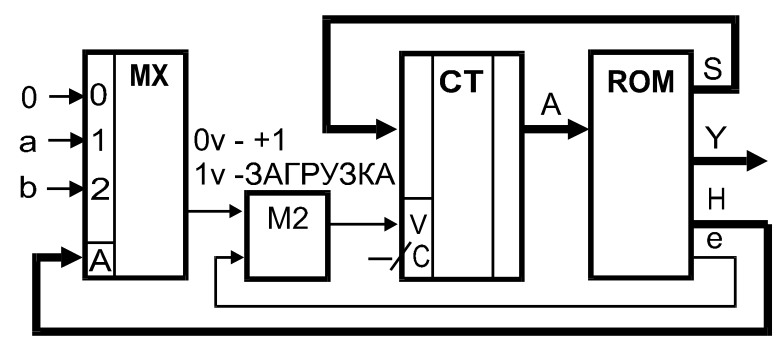
\includegraphics[width=0.5\linewidth]{regular_adress_rom}
		\caption{УА с регулярной адресацией}
		\label{img:scheme}
	\end{center}	
\end{figure}

В конкретной реализации на информационные входы мультиплексора подаются следующие сигналы:
	\hypertarget{name}{}
\begin{itemize}

	\item Константа нуля;
	\item Ma\_IS\_NULL (признак нуля мантиссы А);
	\item Mb\_IS\_NULL (признак нуля мантиссы B);
	\item A<B (признак того, что порядок числа A меньше порядка числа B);
	\item A\_IS\_ANSWER (признак того, что ответ хранится в регистрах числа A);
	\item CT\_dP\_IS\_NULL (признак того, что счетчик разницы порядков хранит "ноль");
	\item CT\_Pa\_IS\_NULL (признак переполнения счетчика порядка числа A в большую сторону);
	\item CT\_Pa\_IS\_MAX  (признак переполнения счетчика порядка числа A в меньшую сторону);
	\item $\left|m\_a\pm m\_b\right|>1$ (признак того, что модуль алгебраической суммы операндов больше единицы);
	\item op\_normalized (признак нормализации операндов);
\end{itemize}

В схему введен элемент М2, позволяющий инвертировать значение входного сигнала, что облегчает распределение микроинструкций по ячейкам управляющей памяти.

\section{Алгоритм работы автомата}
Опишем алгоритм работы автомата с помощью блок схемы. См. рисунок~\ref{img:algorithm} и \ref{img:algorithm2} в \hyperref[tam]{Приложении~А}.

После построения алгоритма работы автомата следует перейти к реализации операционной части.

\section {Реализация Операционного автомата}
Построим операционный автомат, выполняющий сложение двух чисел в формате с плавающей точкой. Приведем названия и назначения каждого из регистров, используемых в данном устройстве. См. таблицу \ref{tab:regs}.
\begin{table}[h!]
	\centering
	\small
		\begin{tabular}{|m{0.27\linewidth}|m{0.6\linewidth}|}
			\hline
			\textbf{Идентификатор} & \textbf{Назначение} \\ \hline
			$RG\_Ma$ & Универсальный сдвиговый регистр. Хранит разряды мантиссы А\\ \hline
			$CT\_Mb$ & Счетчик. Хранит разряды мантиссы B\\ \hline
			$CT\_Pa$ & Счетчик. Хранит разряды порядка числа A \\\hline
			$CT\_Pb$ & Счетчик. Хранит разряды порядка числа B \\ \hline
			$CT\_dP$ & Счетчик. Хранит разряды разницы порядков чисел A и B\\ \hline
			$REG\_SUM$& Триггер. Хранит разряд сигнала переноса суммы мантисс чисел A и B\\\hline
		\end{tabular}
		\caption{Регистры операционного автомата}
		\label{tab:regs}
\end{table}

Укажем необходимые признаки, которые впоследствии будут вырабатываться управляющим автоматом. См. таблицу \ref{tab:signals}.
\begin{table}[h!]
	\centering
	\small
	\begin{tabular}{|m{0.17\linewidth}|m{0.7\linewidth}|}
		\hline
		\textbf{Признак} & \textbf{Назначение} \\ \hline
		$S$ & Хранит адрес следующей операции \\ \hline
		$Н$ & Адресный вход мультиплексора \\ \hline
		$R0$ & Сигнализирует об окончании операции деления \\ \hline
		$overflow$ & Сигнализирует об ошибке обработки -- переполнение \\ \hline
		$L\_Ma$ & Загрузка в регистр $RG\_Ma$ \\ \hline
		$SHIFT\_Ma$ & Правый сдвиг регистра $RG\_Ma$ если $SHIFT\_Ma\_Left=0$ и левый, если  $SHIFT\_Ma\_Left=1$ \\ \hline
		$RST$ & Асинхронный сброс всех элементов \\ \hline
		$COUNT\_Pa$ & Счет. Декремент счетчика, если $L\_CT_\_Pa==1$ \\ \hline
		$L\_CT\_Pa$ & Загрузка счетчика $CT\_Pa$ \\ \hline
		$CHANGE$ & Выбор источника загрузки в регистры мантисс и порядка чисел A и B \\ \hline
		$e$ & Управляющий сигнал для счетчика. Если $e=1$, следует выполнить загрузку, а если $e=0$ -- инкрементировать счетчик. \\ \hline
	\end{tabular}
	\caption{Осведомительные сигналы (признаки)}
	\label{tab:signals}
\end{table}
\newpage
С целью реализации левого и правого сдвига в регистре $RG\_Ma$ был построен элемент памяти, позволяющий выбрать направление сдвига с помощью двух управляющих сигналов. Данный элемент был размещен в отдельном файле и загружался в основной файл как внешняя библиотека Logisim. Устройство данного регистра можно увидеть на рисунке \ref{img:left_reg} в \hyperref[tam]{Приложении А}.

При выполнении операции сложения предполагается, что числа, переданные на вход находятся в нормализованном виде, то есть имеют вид, представленный на сноске \ref{sign}.

\begin{equation}
\begin{aligned}
\label{sign}
\frac12&\le \left|M\right|< 1\\
M &= 0.1XXXX\\
M &= 1.0XXXX\\
M&=1.00000\\
\end{aligned}
\end{equation}

Результат суммы также нормализуется в соответствии с данными правилами. Числа, представленные в ином виде считаются ненормализованными и не обрабатываются цифровым устройством.

Стоит отметить, что для формирования правильного выходного результата необходимо выполнить нормализацию значений суммы в зависимости от вида операндов. Для каждой комбинации операндов реализована отдельная операция нормализации. См таблицу \ref{tab:correction}.

\begin{table}
	\small
	\begin{tabular}{|m{0.3\linewidth}|m{0.67\linewidth}|}
		\hline
		\textbf{Комбинация} &\textbf{Коррекция}\\
		\hline
		 $\left|m_a\pm m_b\right|\ge1$ & Мантисса не нормализована. Сдвинуть регистр мантиссы вправо, загрузить сигнал переноса сумматора. Увеличить порядок результата на 1. При этом может произойти переполнение счетчика в большую сторону \\ 
		\hline
		$\frac12\le \left|m_a\pm m_b\right|< 1$ & Нормализация результата не требуется\\
		\hline
		$\left|m_a\pm m_b\right|<\frac12$ & Мантисса не нормализована. Сдвигая мантиссу влево, уменьшать порядок, при этом может произойти переполнение порядка в отрицательную сторону\\
		\hline
	\end{tabular}
	\caption{Нормализация результата}
	\label{tab:correction}
\end{table}

Соединим все элементы в соответствии с алгоритмом задачи. См. рисунки \ref{img:oa1} и \ref{img:oa2} в приложении \hyperref[tam]{Приложении А}.

\section {Реализация управляющего автомата}
Приступим к построению управляющего автомата, определяющего последовательность выполнения микрокоманд для сложения двух чисел в формате с плавающей точкой.

Определим разрядность ПЗУ, участвующего в построении УА по схеме с постоянной адресацией. Адрес должен иметь 5 разрядов~--- текущее значение параметра \textit{S}. Микрокоманда представлена в виде 22 бит~--- 15 признаков, расположенных в следующем порядке: S,	R0,	RST,	L\_ma,	SHIFT\_Ma,	SHIFT\_Ma\_LEFT,	L\_CT\_Pa,	COUNT\_Pa,	CHANGE,	L\_CT\_dP,	COUNT\_dP,	m\_n,	H,	e. Адрес текущей команды хранится в 5~-ти разрядном счетчике. К входам мультиплексора подлючены сигналы, значения которых анализируются в данном состоянии автомата. Они описаны выше. См. \hyperlink{name}{список}.

Заполним память в соответствии в алгоритмом, подключим ПЗУ, мультиплексор и счетчик последовательным способом. См рисунок \ref{img:ma} в \hyperref[tam]{Приложении А}. 

Ввод и вывод результатов осуществляется с помощью блока ввода и вывода. Числа передаются в нормализованном формате со смещением порядка в С=16. См. рисунок \ref{img:inp_out} в \hyperref[tam]{Приложении A}.


\section {Вывод}
В ходе данной практической работы было рассмотрено строение и работа управляющего автомата, построенного по схеме регулярной адресацией. Использовав полученные знания на практике, на основе данного управляющего автомата построено вычислительное устройство (операционный и управляющий автомат), реализующее операцию сложения двух чисел в формате с плавающей точкой.

\newpage{
\centering
\anonsection{ПРИЛОЖЕНИЕ А}
}
\label{tam}
\begin{figure}[h!]
	\centering
	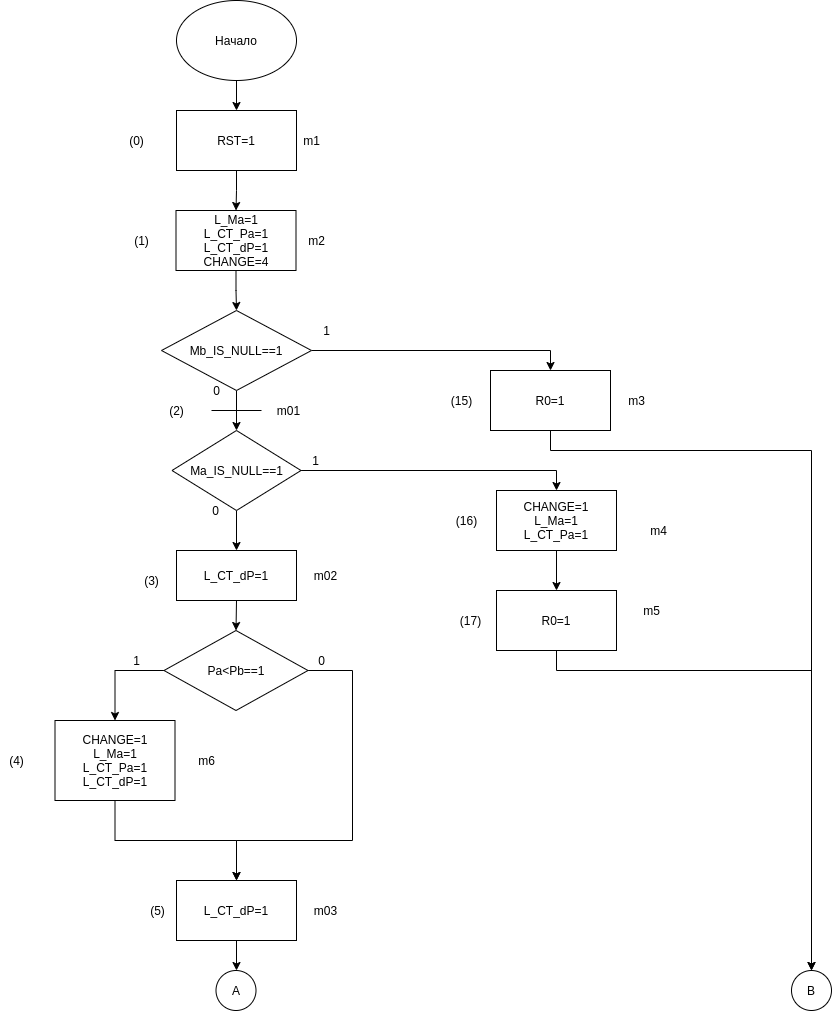
\includegraphics[width=0.7\linewidth]{algorithm5.1}
	\caption {Алгоритм сложения чисел с плавающей точкой. Часть 1}
	\label{img:algorithm}
\end{figure}
\newpage
\begin{figure}[htpb]
	\centering
	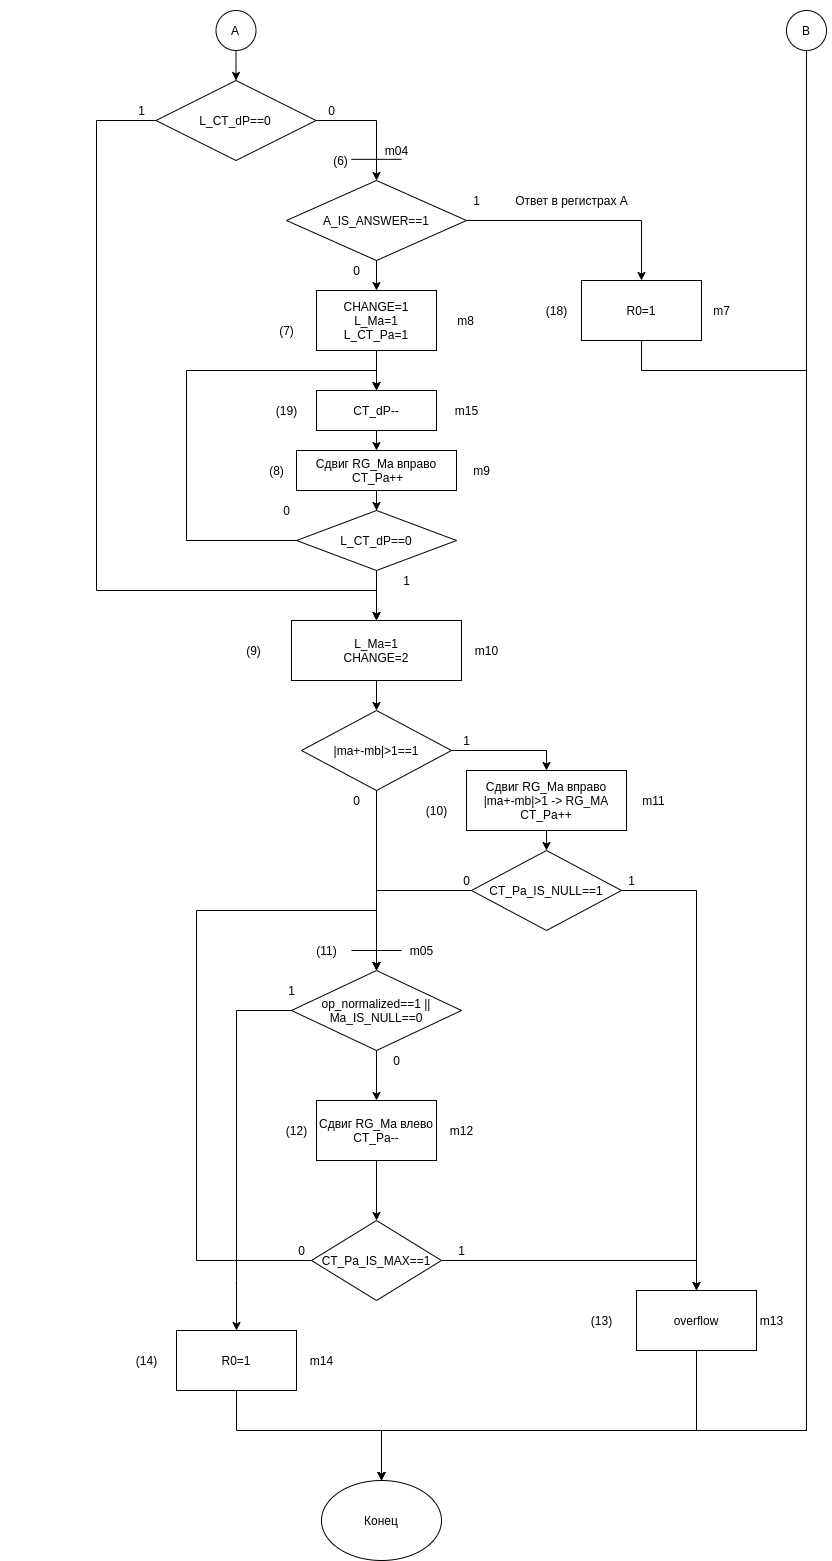
\includegraphics[width=0.5\linewidth]{algorithm5.2}
	\caption {Алгоритм сложения чисел с плавающей точкой. Часть 2}
	\label{img:algorithm2}
\end{figure}
\newpage
\begin{figure}[htpb]
	\centering
	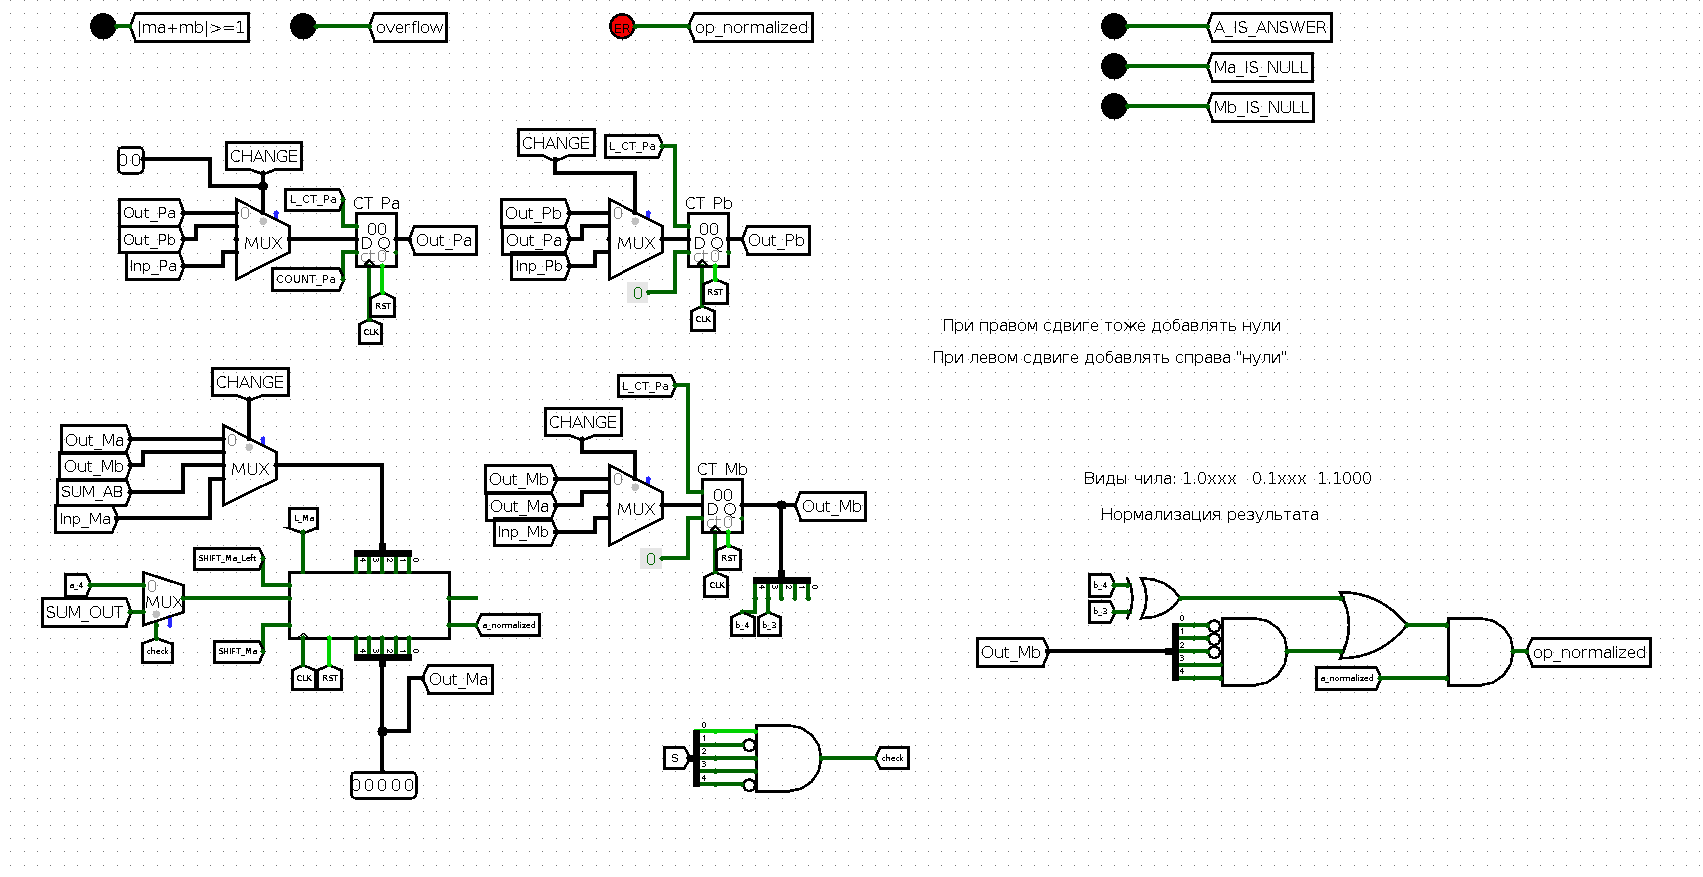
\includegraphics[width=0.9\linewidth]{oa5.1}
	\caption {Схема операционного автомата, часть 1}
	\label{img:oa1}
\end{figure}
\begin{figure}[htbp]
	\centering
	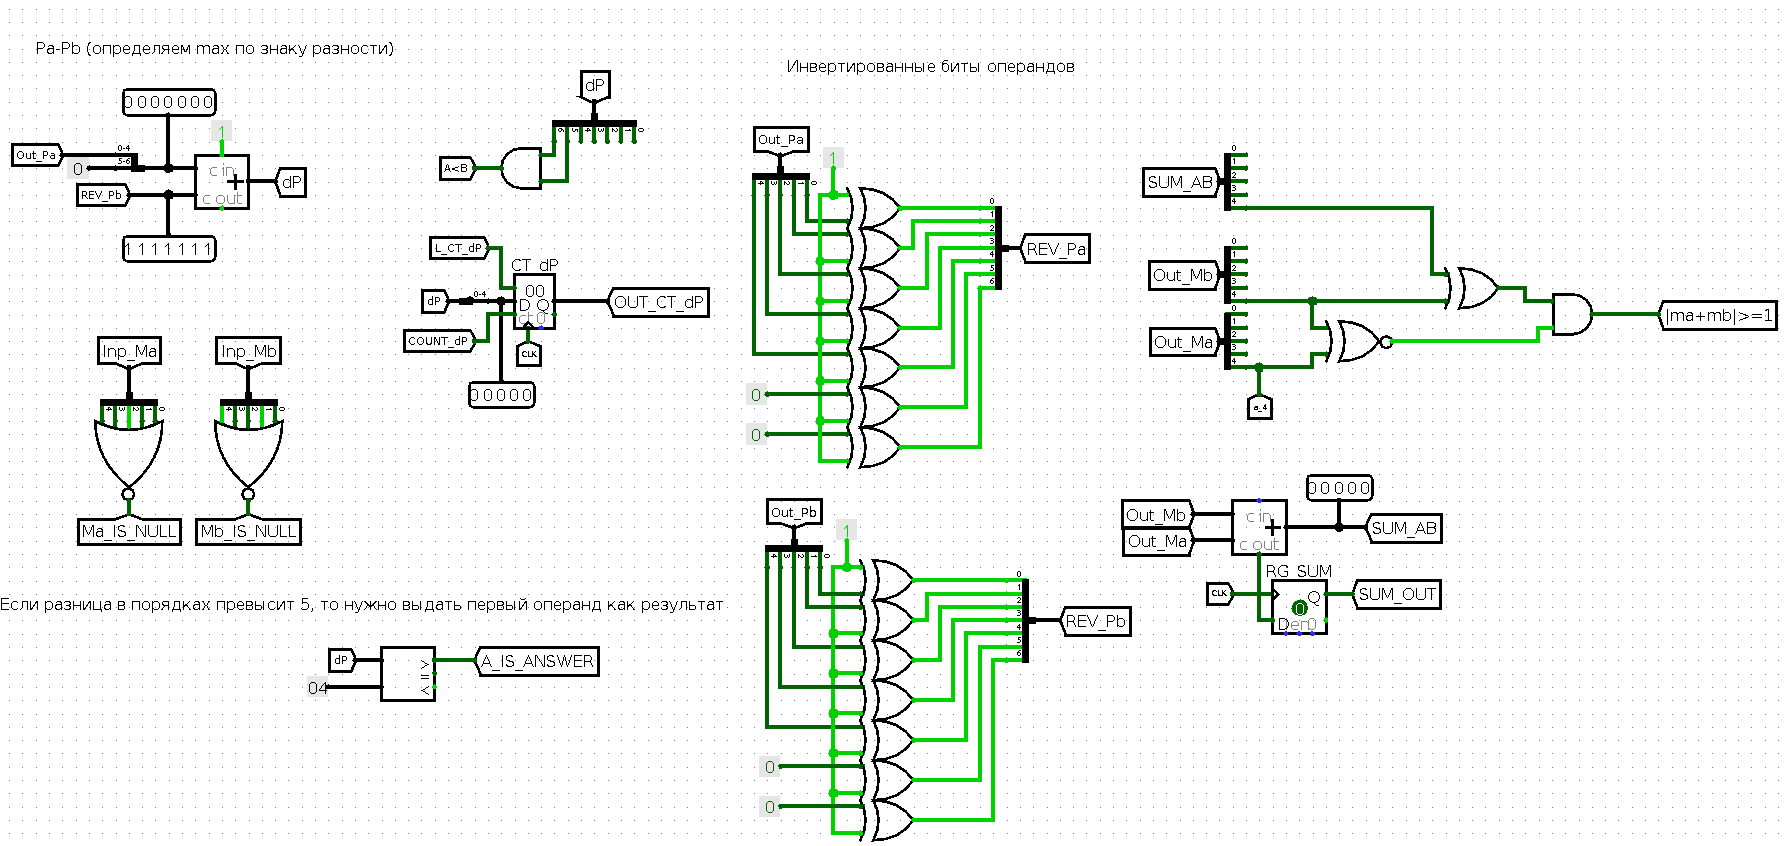
\includegraphics[width=0.9\linewidth]{oa5.2}
	\caption {Схема операционного автомата, часть 2}
	\label{img:oa2}
\end{figure}

\begin{figure}[htbp]
	\centering
	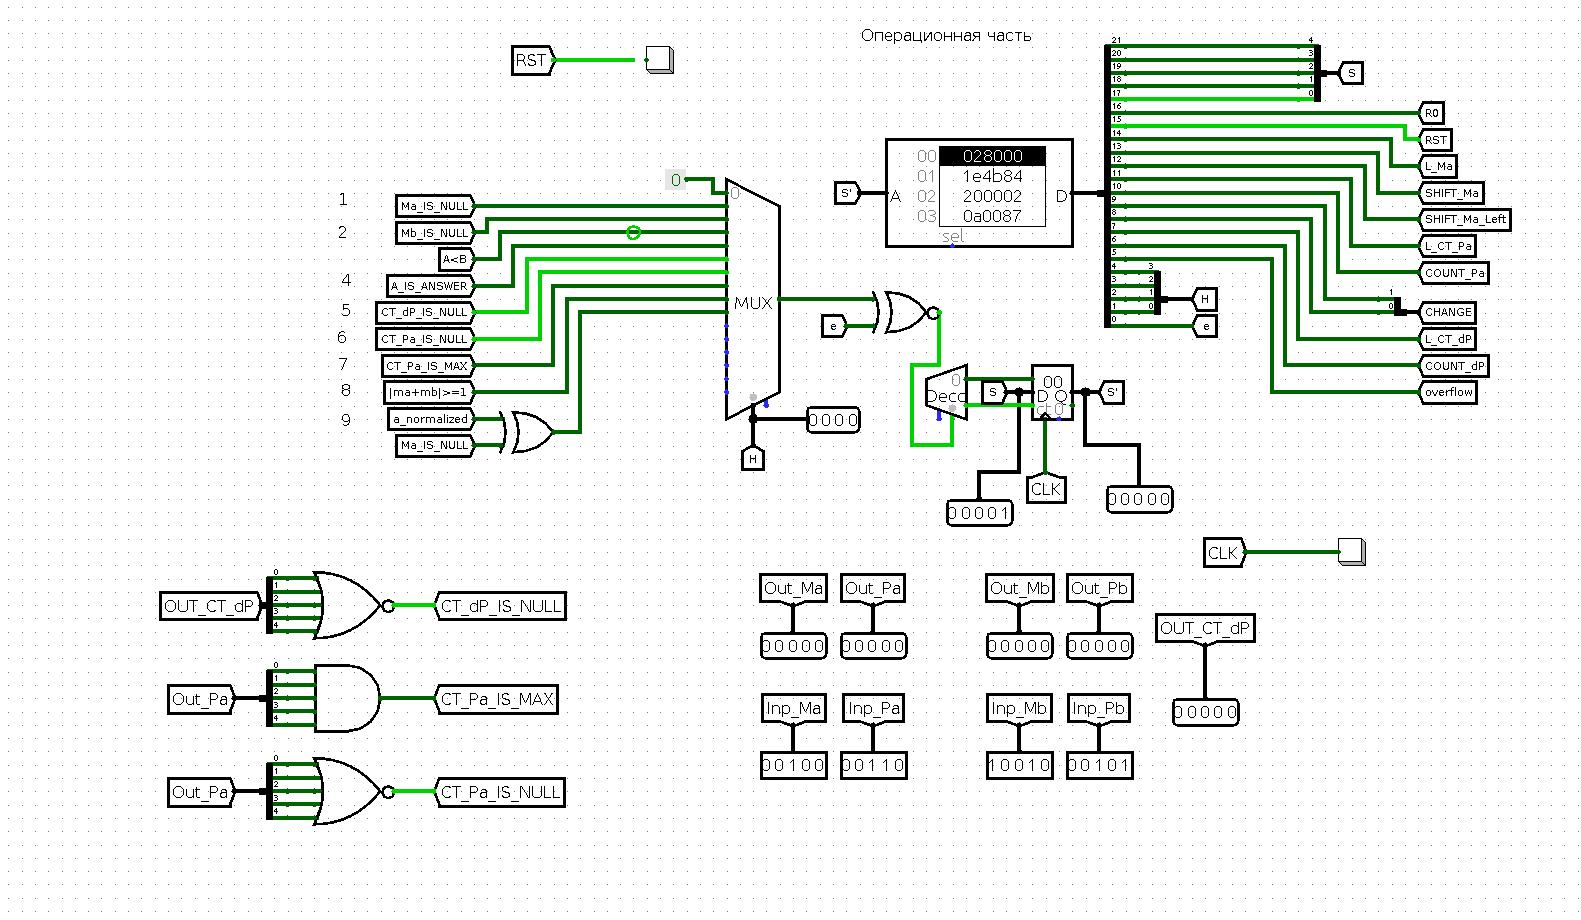
\includegraphics[width=\linewidth]{ma5}
	\caption {Схема управляющего автомата}
	\label{img:ma}
\end{figure}

\begin{figure}[htbp]
	\centering
	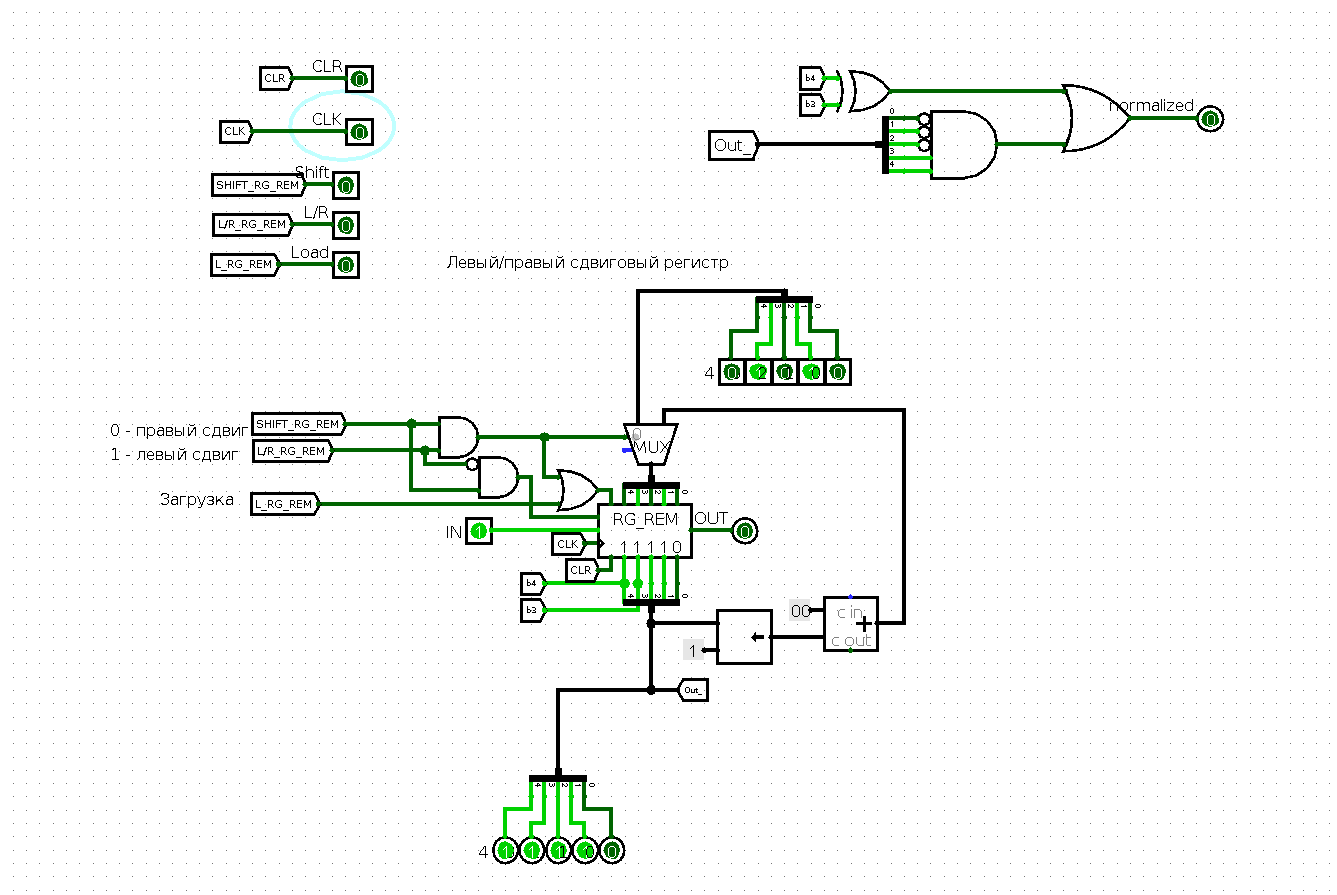
\includegraphics[width=\linewidth]{left_reg}
	\caption {Устройство универсального регистра}
	\label{img:left_reg}
\end{figure}

\begin{figure}[htbp]
	\centering
	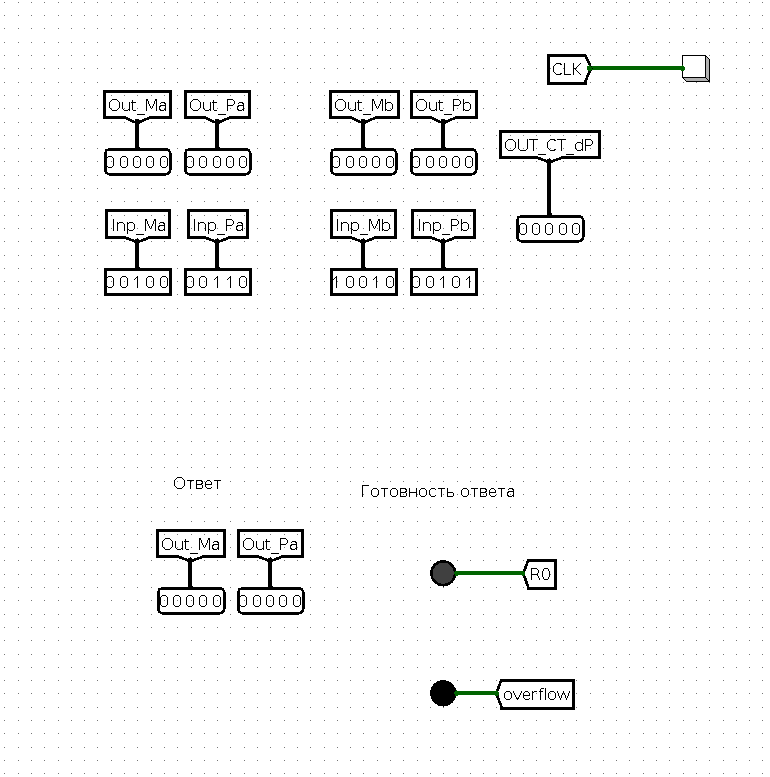
\includegraphics[width=\linewidth]{inp_out}
	\caption {Блок ввода-вывода}
	\label{img:inp_out}
\end{figure}

\end{document}


